\documentclass{article} % For LaTeX2e
\usepackage{nips15submit_e,times}
\usepackage{hyperref}
\usepackage{url}
\usepackage[pdftex]{graphicx}
\usepackage{float}
\usepackage{amsmath}
\usepackage{amssymb}
%\documentstyle[nips14submit_09,times,art10]{article} % For LaTeX 2.09


\title{Information Retrieval and DataMining:\\
		Memory Models for Time Series Analysis
}


\author{
Mark Neumann, Alexander Chapovskiy and Zheng Tian\\ %thanks{} \\
UCL\\
\texttt{mark.neumann.15@ucl.ac.uk} \\
\texttt{alexander.chapovskiy.15@ucl.ac.uk} \\
\texttt{zheng.tian.11@ucl.ac.uk@ucl.ac.uk} \\
}
\newcommand{\fix}{\marginpar{FIX}}
\newcommand{\new}{\marginpar{NEW}}
\newcommand{\be}{\begin{equation}}
\newcommand{\ee}{\end{equation}}
\newcommand{\Ermse}{E_{\rm \scriptsize rmse}}
%\DeclareMathOperator*{\tanh}{tanh}


\nipsfinalcopy % Uncomment for camera-ready version

\begin{document}


\maketitle
\graphicspath{{images/}}

\begin{abstract}
This is a report for group project in the Information Retrieval and Data 
Mining course. In this report we investigate different deep neural network
architectures on the time series. In particular, we apply neural 
networks to energy load and household energy consumption datasets.
\end{abstract}


\section{Introduction}
\label{sec:intro}

\subsection{Memory Models}
Long Short-Term memory\cite{LSTM} has been utilised widely across many disciplines in Machine Learning, with particularly notable performance in domains such as Machine Translation\cite{Sutskever}, Constituency Parsing\cite{Parsing}, Speech Recognition and even generative models, such as human level handwriting generation.\cite{Graves} 

Particularly key in the success of LSTM and other variants, such as the GRU, has been their perceived ability to selectively encode long-term dependencies and learn precise timings. In this work, we investigate the effect of precise timings in accurately modelling time-series data, an area which should particularly benefit from the accuracy features provided by Long Short-Term memory.

\subsection{Other Model Architectures}

One perceived failure of neural networks until recently was their inability to deal with arbitrary sequence lengths. The input dimensions to a standard LSTM classifier/regressor are fixed, meaning that data which intrinsically contains irreducible sequences of different lengths was difficult or impossible to process. This clearly is a problem with time series data, as the noisy nature of real world data means that we are rarely going to achieve perfectly timed and sanitised data.

In \cite{Sutskever}, Sutskever introduces sequence to sequence neural networks, which utilise two separate networks, one to encode a sentence into a vector representation and the other to decode a vector representation into the model ouptut. These are trained jointly, enabling arbitrary length sequences and particularly enabling non-monotonic transformations. We note that although we do not explore sequence to sequence models in this paper, the underlying cell structure we explore can be used in this architecture and that this is a very interesting area of development for time series models given their nature.  

{\LARGE \color{red} THIS PAPER IS ORGENISED AS FOLLOWS!!!!!!}



\section{Recurrent Neural Networks}
\label{sec:nn}

Below we describe the models applied to the dataset, for which performance can be found in the next section. In addition to vanilla Long Short-Term Memory, we explore several recent innovations over the last few years, including Gated Recurrent Units and peephole connections. 



\subsection{LSTM}
\label{sec:nn/lstm}


Given an input vector $x_{t} \in \mathbb{R}^{N}$ at time $t$ and the previous output of the LSTM $h_{t-1} \in \mathbb{R}^{K}$, the forget gate($f_{t}$), the input gate($i_{t}$), the output gate($o_{t}$) and the cell input($z_{t}$) are computed as follows:
\begin{equation}
\begin{aligned}[c]
    H &= \left[ \begin{array}{cc}
         x_{t}  \\
         h_{t-1} 
    \end{array} \right] \in \mathbb{R}^{N+K} \\
    z_{t} &= Tanh(W_{z}H + b_{z}) \\
    i_{t} &= \sigma(W_{i}H + b_{i})\\
    \end{aligned}
    \qquad \qquad
    \begin{aligned}[c]
    o_{t} &= \sigma(W_{o}H + b_{o})\\
    f_{t} &= \sigma(W_{i}H + b_{i})\\
    c_{t} &= f_{t} \odot c_{t-1} + i_{t} \odot z_{t} \\
    h_{t} &= o_{t} \odot Tanh(c_{t}) \\
    \end{aligned}
\end{equation}

Where $W_{z}, W_{i}, W_{o}, W_{f} \in \mathbb{R}^{K \times(N+K)}$ and $b_{z}, b_{i}, b_{o}, b_{f} \in \mathbb{R}^{K}$ are trained weight matrices and bias vectors for $N$, the dimension of the input vector and $K$ the hidden size of the LSTM. $\sigma$ and $Tanh$ are element-wise activation functions representing the sigmoid and hyperbolic tangent functions, with $\odot$ representing element-wise multiplication. 

Below we present a pictorial demonstration of the connections in the LSTM cell. 

\begin{figure}[H]
\begin{center}

\includegraphics[width=0.8 \linewidth]{LSTM.png} 
\end{center}
\caption{A demonstration of the interactions within an LSTM cell. Here we can see clearly how the input and output control the respective features of the cell: the closer to zero these vectors are, the smaller the amount of information which can travel through the dot product.}
\end{figure}




\subsection{Gated Recurrent Unit}
\label{sec:nn/gru}

The Gated Recurrent Unit\cite{DBLP:journals/corr/ChungGCB15} can be seen as a simplified LSTM with a tied output and forget gate, merging two of the above equations. 

Given an input vector $x_{t} \in \mathbb{R}^{N}$ at time $t$ and the previous output of the GRU $h_{t-1} \in \mathbb{R}^{K}$, the forget gate($f_{t}$), the input gate($i_{t}$) and cell output($h_{t}$)  are computed as follows:
\begin{equation}
\begin{aligned}[c]
         &Input: x_{t}  \\
         &Prev State: h_{t-1} \\
    	 &i_{t} = \sigma(W_{i}^{x}x_{t} + W_{i}^{h} h_{t-1} + b_{i})\\
    \end{aligned}
    \qquad \qquad
    \begin{aligned}[c]
    f_{t} &= \sigma(W_{f}^{x}x_{t} + W_{f}^{h} h_{t-1} + b_{f})\\
    \tilde{h_{t}} &= Tanh(W x_{t} + f_{t} \odot h_{t-1})\\
    h_{t} &= i_{t} \odot h_{t-1} + (1- z_{t}) \odot \tilde{h_t}  \\
    \end{aligned}
\end{equation}

Where $W_{i}^{x}, W_{f}^{x}, \in \mathbb{R}^{K \times(N)}, W_{i}^{h}, W_{f}^{h} \in \mathbb{R}^{K \times(K)}$ and $b_{i} \in \mathbb{R}^{N}, b_{f} \in \mathbb{R}^{K}$ are trained weight matrices and bias vectors for $N$, the dimension of the input vector and $K$ the hidden size of the GRU. $\sigma$ and $Tanh$ are again element-wise activation functions representing the sigmoid and hyperbolic tangent functions, with $\odot$ representing element-wise multiplication as above. 

It should be noted that subsequent papers by Cho expand on the GRU, particularly to incorporate "recurrent feedback", intuitively described as a linear combination of memory storage across hidden layers. This would certainly be an interesting extension to the work in this paper.


\subsection{Peephole Connections}
\label{sec:nn/peephole}

Peephole connections are a popular addition to the Long Short-Term memory model\cite{peepholeconnections}. Originating in a paper by Schmidhuber and Gers whilst working at the IDSIA lab in Switzerland, they quickly became popular in an array of literature. The basic premise is that the gates of the LSTM mechanism become a function not only of the current input $x_{t}$ and previous LSTM state $h_{h-1}$, but also a function of the current cell memory state which persists from the last timestep,  $c_{t-1}$. The input, output and forget gates are therefore defined as follows:

\begin{equation}
\begin{aligned}[c]
 H &= \left[ \begin{array}{cc}
         x_{t}  \\
         h_{t-1} \\
         c_{t-1}
    \end{array} \right] \in \mathbb{R}^{N+2K} \\
\end{aligned}
\qquad \qquad
    \begin{aligned}[c]
    i_{t} &= \sigma(W_{i}H + b_{i})\\
    f_{t} &= \sigma(W_{f}H + b_{f})\\
    o_{t} &= \sigma(W_{o}^{x}x_{t} + W_{o}^{h}h_{t-1} + W_{o}^{c}c_{t} +  + b_{o})\\
    \end{aligned}
\end{equation}

where the memory is simply appended onto the vector used in the LSTM mechanism for the calculation of the input and forget gates, with the output gate using a different format only because it uses the {\it current} state's memory, rather than the previous one as in the input and forget gates. The other functionality remains unchanged. Additionally, some practitioners choose to only apply peephole connections to gates selectively - often, they are only applied to the input and output gates and not the forget gate. Note the effect of peephole connections is difficult to measure accurately, as in a vanilla LSTM, all the gates are implicitly a function of the memory vector, as they are a function of the previous state which is informed by the memory at that point. Below we present a pictorial representation of how the addition of peephole connections changes the internal cell architecture.

\begin{figure}[H]
\begin{center}
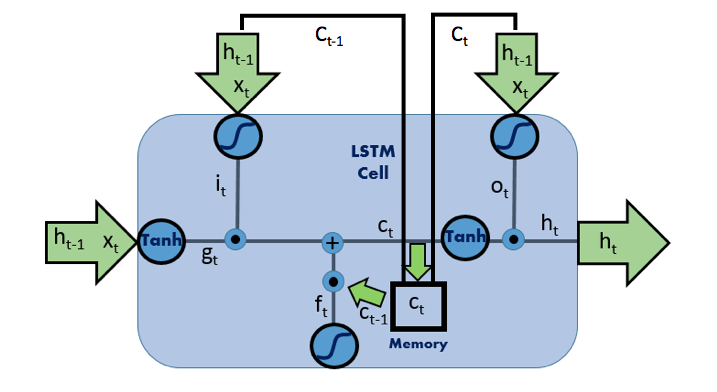
\includegraphics[width=0.8 \linewidth]{LSTM_Peepholes.png} 
\end{center}
\caption{Here we can clearly see how all gates now have direct interaction with the memory state.}
\end{figure}



\section{Datasets}
\label{sec:data}


\subsection{Energy Load}
\label{sec:data/energy}

In this section we describe a dataset of Energy Load.
The dataset contains energy load for 20~power stations over approximately 4~years
every hour with some weeks missing. 
The dataset also provides temperatures at 11~weather stations. It is clear that
there must be correlation between temperature and energy load.
However, one of the difficulties is that it is unknown
which temperature corresponds to which power station. As a matter of fact, 
it is possible that weather station is located between two power stations
and is therefore relevant for both. 

This dataset was used in the Kaggle competition. 
The competition required a prediction of energy load for the missing weeks
using temperatures available during, and 
temperatures and loads before and after missing weeks. It also required 
prediction for the week immediately after the end of the dataset
with no temperature available. 
As it is unknown which temperature reading is relevant for a particular
power station, the competition also required to
determine the relevance of weather stations for a particular power station
statistically.
Here our goal is to investigate application of neural networks to time series data.
Therefore we focus on one week ahead prediction of the energy load 
at each of 20~power stations
using temperatures during that period and temperatures and loads prior to 
that week.

After the competition
the winners of the competition published their approaches, 
\cite{energy_kaggle}.
Mostly the approaches were based on linear regression with 
hand crafted non-linear features using various improvements
such as, for example, gradient boosting.
In Section~\ref{sec:energy} we apply a regression model with 
handcrafted non-linear features to serve as a benchmark.
We then discuss deep feed-forward Neural Network with simple
variables, such as temperature, day of the week, hour, {\it etc},
for week ahead prediction to see if the network is able to discover
relevant features. 
We then discuss a Recurrent Neural Network, which additionally takes
prior week loads and temperatures, in order to see if RNN is able to 
discover additional regularities, not captured by the variables above.




\subsection{Household Energy Consumption}
\label{sec:data/house}

{\LARGE \color{red} !!!Description of the dataset}




\section{Prediction of Energy Loads}
\label{sec:energy}

In this section we discuss different models applied to the Energy Load dataset
described in Section~\ref{sec:data/energy}.
We first discuss a simple regression model with non-linear features
in Section~\ref{sec:energy/reg}, which serves as a benchmark for more 
complicated models.
In Section~\ref{sec:energy/nn} we apply deep neural network with simple inputs
to the dataset in order to see if the network is able to find relevant 
non-linear features.
In Section~\ref{sec:energy/rnn} we apply Recurrent Neural Network,
with prior week's temperatures and load as inputs, to the dataset
in order to see if the network is able to find some additional
regularities in the historical information.

In order to compare the performance of different models we formulate the 
problem in the following way. We split all the data into overlapping
2~week periods, each week from Monday to Sunday.
In each pair of weeks the goal is to predict energy loads for 20~stations
in the second week
using temperatures from 11~weather stations in the second week and 
energy loads and temperatures in the first week. 
Thus, for every pair of weeks 
we have to make $20\times7\times24$ load predictions.
This way we have about 200 week-pairs in total.
We allocate 20\% of the data for testing, with remaining 80\%~of the 
data used for training and validation.
We optimise all models using mean square error objective function
\begin{equation}
	E_{\rm\scriptsize mse} = 
	\frac{1}{N}\sum_i \biggl(
	L_{\rm\scriptsize predicted}^{(i)}-
	L_{\rm\scriptsize actual}^{(i)}\biggr)^2,
\end{equation}
where $L_{\rm\scriptsize predicted}^{(i)}$
and $L_{\rm\scriptsize actual}^{(i)}$ are predicted and actual
energy load respectively and the sum is over all week, week day, hour, zone
combinations.
For convenience we compare performance of different models using dimensionless
measure (relative square root of mean square error)
\begin{equation}
	\Ermse =
	\frac{\sqrt{E_{\rm\scriptsize mse} }}{\overline{L}_{\rm\scriptsize actual}}, 
\end{equation}
where $\overline{L}_{\rm\scriptsize actual}$ is the average load
over the entire dataset.


\subsection{Features and Regression Model}
\label{sec:energy/reg}

In order to construct a baseline to examine our results, we perform 
linear regression with non-linear features on batches of one week's worth of data.
It is natural to expect that energy load in zone, $L_z(t)$, 
is a function of 
hour, $h$, week day, $w$, and temperature at all weather stations, $T_i$,
as it is not know which weather station is relevant for zone $z$.
It is also natural to expect that the load is correlated with the load 
at the same zone during the prior week.
Therefore we use the following features
\begin{itemize}
	\item {\bf Bias}.
	\item {\bf Temperature}. We use linear and quadratic features, $T_i$ 
	and $T_i^2$, for all weather stations, $i$.
	\item {\bf Hour}. We use features up to the third power, $h$, $h^2$
	and $h^3$.
	\item {\bf Day of the week}. We use linear and quadratic features,
	$w$ and $w^2$.
	\item {\bf Previous Load}. 20~zone loads averaged over the previous week.
\end{itemize}
Thus we have 48~features in total.

\begin{figure}[h]
\begin{center}
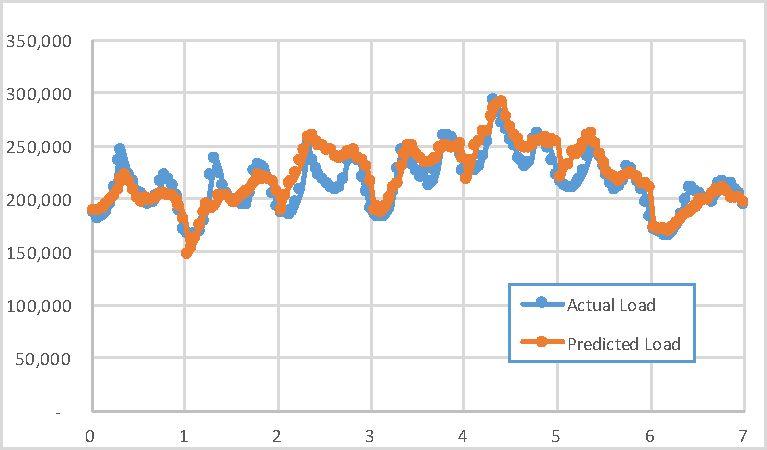
\includegraphics[width=0.45\linewidth]{energy_reg1.pdf}	
\ \ \ 
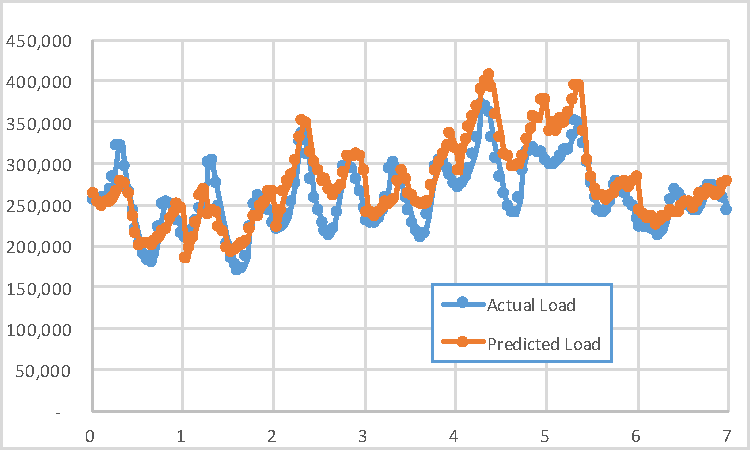
\includegraphics[width=0.45\linewidth]{energy_reg2.pdf}	
\end{center}
\caption{Predicted and actual energy loads for two different weeks and zones.
Prediction is done by regression model.}
\label{fig:energy/reg}
\end{figure}
We calculate feature vector for every every week/week-day/hour 
combination, normalise the 
feature vector over the data and 
run regularised regression on normalised feature vector.
The output of the regression is 20-dimensional vector of energy load predictions
for every zone and every week/week-day/hour. 
We obtain relative error of $\Ermse=(15\%,16\%)$ 
for training and test sets respectively%
\footnote{
The model is implemented in {\tt model\_reg.py}.
}. 
The errors for training and test sets 
are the same indicating lack of over-fitting.
Fig.~\ref{fig:energy/reg} shows predicted and observed energy loads
for two different zones and weeks. One can see that our simple regression
model, while not perfect, captures roughly the behaviour of the 
energy loads.

\subsection{Feed-Forward Neural Network}
\label{sec:energy/nn}

In Section~\ref{sec:energy/reg} we implemented a simple regression model
with non-linear features. There we chose non-linear features by hand using
domain knowledge. In this section we implement a deep  feed-forward
neural network in order to see if the networks will be able to find 
relevant features automatically.

\begin{figure}[h]
\begin{center}
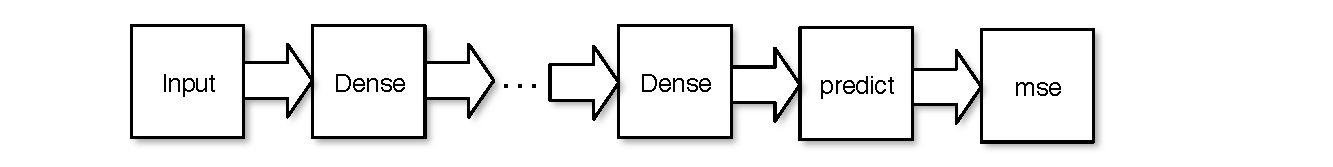
\includegraphics[width=1\linewidth]{energy_NN_diag.pdf}	
\end{center}
\caption{Architecture of feed-forward neural network.}
\label{fig:energy/nn_diag}
\end{figure}
Fig~\ref{fig:energy/nn_diag} shows schematically the architecture of the model.
Different elements are the following
\begin{itemize}
	\item {\bf Input}.
	The input contains the following information: week-day, hour, 11~temperatures
	at the same hour, energy load averaged over the previous week 
	for 20~zones. There are 33~inputs in total.
	\item {\bf Dense}. 
	The input is passed to a series of standard fully connected layers with
	{\tt ReLu} non-linearity. By looking at the validation set error
	we found that $8$~dense fully connected layers each with dimension~33,
	the same as the input dimension,works the best.
	\item {\bf Predict}.
	The output of the dense network is passed to 20-dimensional 
	prediction layer.
	\item {\bf MSE}.
	Mean square loss objective, which is minimised. 
\end{itemize}
Minimization of all the weights is performed by
stochastic gradient decent.
Implementation%
\footnote{
Implementation of the model can be found in directory {\tt KerasRNN}
in {\tt model1\_2.py}, which is used by {\tt train1.py}.
} is using Keras/Theano for NN code, which relies on Cuda to run
on GPU.
As before we use 20\% of the whole data for final testing (7,056 observations). 
The remainder we split into 20\% for validation set (5,544 observations), 
and the rest is used as a training set (2,2848 observations).


\begin{figure}[h]
\begin{center}
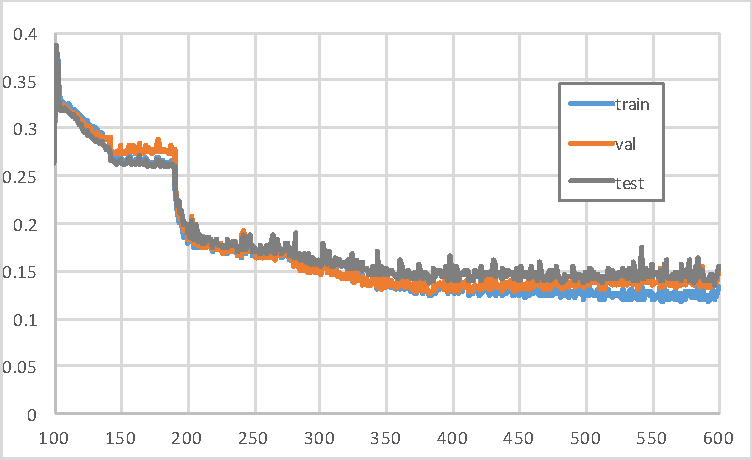
\includegraphics[width=0.7\linewidth]{energy_NN_learning.pdf}	
\end{center}
\caption{Relative error as function of learning epoch for training, 
validation and test data.}
\label{fig:energy/nn/learn}
\end{figure}
Fig.~\ref{fig:energy/nn/learn} shows relative error as function of 
learning epoch for training, validation and test data.
One can see that in the very end training and validation errors start to diverge.
We adopt early stopping by monitoring validation set error.
At the minimum of validation error we obtain errors $(12.5,12.5,13.5)\%$
for training, validation and test sets respectively.
Thus should be compared with $(15,16)\%$ errors for training and test sets
we obtained with regression. NN performance is slightly better.
Thus we can conclude that NN did not only find the hand-made features we used
in regression, but also some additional features, which we missed.


\subsection{Recurrent Neural Network}
\label{sec:energy/rnn}

In Section~\ref{sec:energy/nn} we discussed a fully connected feed-forward
neural network, which managed to discover non-linear dependence
of load as a function of hour, week day, temperature, and average load in 
the previous week. Average load in the previous week was one of the inputs,
which we had to provide explicitly. In this section we discuss
Recurrent Neural Network to which we pass the previous week's history
as an input. 
We would like to see if the network is able to automatically find relevant 
features of the history useful for predicting the load.


\begin{figure}[h]
\begin{center}
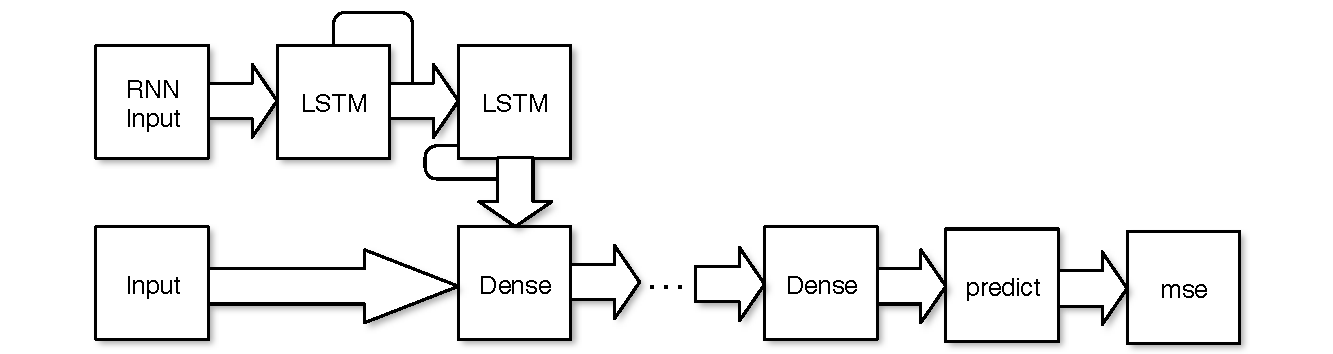
\includegraphics[width=1\linewidth]{energy_RNN_diag.pdf}	
\end{center}
\caption{Architecture of RNN with feed-forward neural network.}
\label{fig:energy/rnn_diag}
\end{figure}
Fig.~\ref{fig:energy/rnn_diag} shows the architecture of the network.
\begin{itemize}
	\item {\bf Input}.
	The input contains the following information: week-day, hour, 11~temperatures
	at the same hour. There are 13~inputs in total. Note, that we do not provide
	average of the history as before.
	\item {\bf RNN Input}.
	Here we would like to provide the whole previous week history of 
	loads and temperatures. However, there are $24\times7=168$ observations,
	which makes RNN network very deep and we were not able to successfully
	train it. In order to overcome this difficulty, we pass 7~loads and 
	temperatures averaged over each day of the previous week. 
	This way he hope the network will discover regularities over the previous
	week but not intra-day.
	Thus 
	RNN input consists of
	7~$(20+11)$-dimensional vectors.
	\item {\bf LSTM}. RNN input is passed to two LSTM layers with 
	$2\times(20+11)=62$ hidden states. Each LSTM uses $tanh$ non-linearity.
	\item {\bf Dense}. 
	Output of LSTM layer is combined with Input and is passed to a series of dense
	layers, similar to Section~\ref{sec:energy/nn}. 
	By looking at validation error we found that 4 dense layers,
	each layer having $2\times(20+11)+13=44$ states,
	works pretty well. Each Dense layer has {\it ReLu} non-linearity.
	\item {\bf Predict}.
	The output of the dense network is passed to 20-dimensional 
	prediction layer.
	\item {\bf MSE}.
	Mean square loss objective, which is minimised. 
\end{itemize}


\begin{figure}[h]
\begin{center}
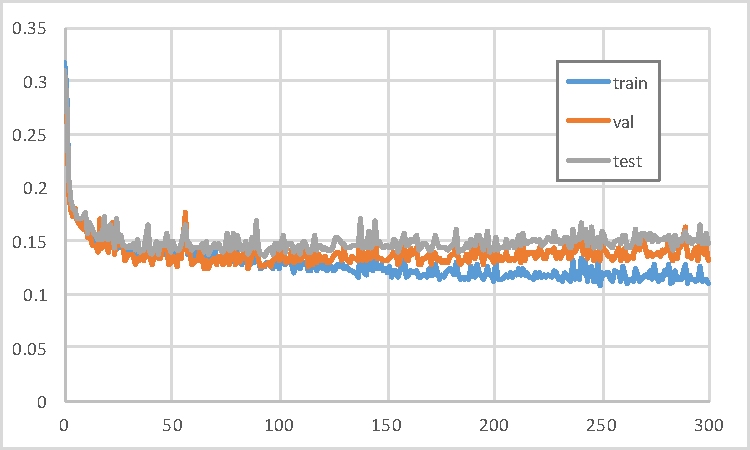
\includegraphics[width=0.70\linewidth]{energy_RNN_learning.pdf}	
\end{center}
\caption{Error of the RNN-dense network as function of training epoch for 
training, validation and test sets.}
\label{fig:energy/rnn_learn}
\end{figure}
We implemented%
\footnote{
Implementation can be found in directory {\tt KerasRNN} in 
file {\tt  model2\_1.py},
which should be used together with {\tt train2.py}
}
this model using Keras/Theano for neural network implementation, which in turn 
uses Cuda for GPU calculations. The network is trained using stochastic 
gradient decent.
Fig.~\ref{fig:energy/rnn_learn} shows dependence of the relative 
mean square error as a function of training epoch for training, validation 
and test sets. One can see that three curves converge very quickly and
are generally close to each other. In the later stages of the training they
exhibit slight over-fitting, so we apply early stopping by monitoring
validation error. We obtain errors of $(13,12.5,13.5)\%$ for training,
validation and test sets respectively.
This should be compared with  $(12.5,12.5,13.5)\%$ we obtained
with NN in Section~\ref{sec:energy/nn}. One can see that results are comparable.
This means that our RNN managed to find the only relevant feature from the history,
which is the average load over the previous week.
This is quite disappointing as the model is quite a bit more complicated.
However, it is quite possible that dependence on the history 
(additionally to average) is not large in our dataset.
Also, it does find the average load, which was provided by hand previously,
which is quite satisfying, as in principle this was not guaranteed.

\begin{figure}[h]
\begin{center}
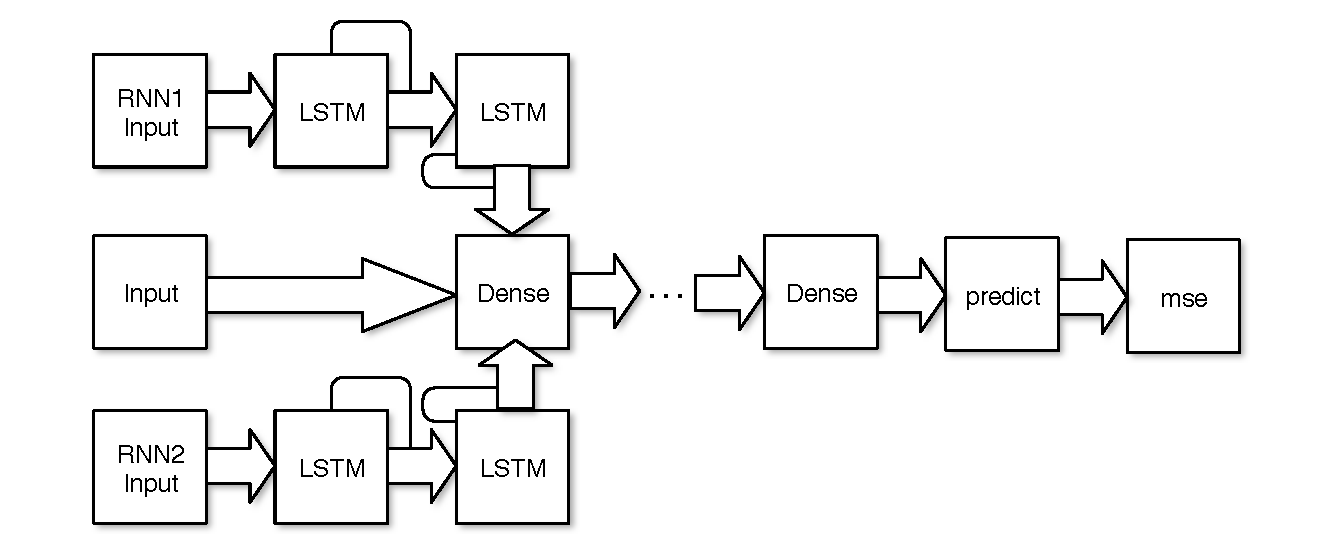
\includegraphics[width=1\linewidth]{energy_RNN2_diag.pdf}	
\end{center}
\caption{Architecture of double-RNN with feed-forward neural network.}
\label{fig:energy/rnn2_diag}
\end{figure}
It has to be noted that in the calculations above we made an approximation.
Instead of passing all $24\times7$ $(20+11)$-dimensional vectors,
which we could not do for computational reasons,
we  pass $7$, each representing average over each day of the week.
In this way we hoped that the network would find {\it "long range"}
regularities on the scale of the week. It is possible that there are
regularities, which are lost, when averaging intra-day. For example,
it is possible that load over a day has some particular structure,
which would help prediction.
In order to investigate this dependence we implemented%
\footnote{
Implementation can be found in directory {\tt kerasRNN} in file
{\tt model.py} to be used with {\tt train.py}.
}
a model with architecture shown in Fig.~\ref{fig:energy/rnn2_diag}.
In that model we have three different inputs: Input and RNN1 Input
are as before. RNN2 Input is new and consists of 24 $(20+11)$ dimensional 
vectors representing average load and temperature over the previous week 
for every hour. RNN2 input is passed to its own LSTM layer, which is 
then combined with the rest of the network and fed into dense layers,
like before.
We do not give further details of the calculations because, although
this model produces results comparable to what we obtained before, 
unfortunately, it does not result in any significant improvements.
Again, it is possible that there is no any further signal from history
due to the nature of the data. On the other hand, this version of the model
is quite a bit more complicated and is harder to train.




\section{Prediction of Household Energy Consumption}
\label{sec:house}




\section{Conclusions}
\label{sec:conclusions}

{\LARGE \color{red} ADD CONCLUSIONS !!!}

Overall, we have examined the performance of peephole connections and neural network architectures in general for several tasks, drawing mixed results. 




\begin{thebibliography}{9}


\small{



\bibitem{DBLP:journals/corr/ChungGCB15}

Junyoung Chung and
               {\c{C}}aglar G{\"{u}}l{\c{c}}ehre and
               KyungHyun Cho and
               Yoshua Bengio (2014)
{\it Gated Recurrent Neural Networks}

\bibitem{peepholeconnections}

Gers, F. and Schmidhuber, J. (2000)
{\it  Recurrent Nets that time and Count} 

\bibitem{Sutskever}

Sutskever, I., Vinyals, O., Le, Q.V. (2015)

{\it Sequence to Sequence Learning with Neural Networks}


\bibitem{Graves}
Graves, A. (2013)
{\it Generating Sequences With Recurrent Neural Networks}

\bibitem{Parsing}
Oriol Vinyals and
               Lukasz Kaiser and
               Terry Koo and
               Slav Petrov and
               Ilya Sutskever and
               Geoffrey E. Hinton, (2015)
{\it Grammar as a Foreign Language}

\bibitem{LSTM}

Sepp Hochreiter and Jürgen Schmidhuber(1995)
{\it Long Short-Term Memory}

\bibitem{energy_kaggle}
Tao Hong, Pierre Pinson and Shu Fan, 
(2014), {\it Global Energy Forecasting Competition 2012.}
International Journal of Forecasting, 30(2), 357;
\\

Charlton, N. and Singleton, C. 
(2014). 
{\it A refined parametric model for short term load forecasting.}
International Journal of Forecasting,
30(2), 364-368.
\\
Souhaib Ben Taieba and Rob J. Hyndmanb,
(2014), 
{\it A gradient boosting approach to the Kaggle load forecasting 
competition.}
International Journal of Forecasting, 30(2), 382;
\\
Lloyd, J. R. (2014), 
{\it GEFCom2012 hierarchical load forecasting: Gradient boosting machines and Gaussian processes. }
International Journal of Forecasting, 30(2), 369.


}

\end{thebibliography}

\end{document}
